\documentclass[preprint,review,12pt]{elsarticle}

\usepackage[T1]{fontenc}
\usepackage{lmodern}
\usepackage{microtype}
\usepackage{amsmath}
\usepackage{graphicx}
\usepackage{booktabs}
\usepackage{tabularx}
\usepackage{siunitx}
\setlength{\marginparwidth}{2cm}
\usepackage[colorinlistoftodos]{todonotes}

\newcommand{\zy}[1]{\todo[color=blue!20]{Ziyu: #1}}
\newcommand{\thom}[1]{\todo[color=orange!25]{Thom: #1}}
\newcommand{\inlinecomment}[1]{\todo[inline,color=yellow!30]{#1}}

\journal{Acta Astronautica}
\graphicspath{{figures/}}
\sisetup{detect-all}
\setlength{\emergencystretch}{2em}
\hfuzz=3pt

\begin{document}

\begin{frontmatter}

\title{Benchmarking foundation models for reactive
EMI--BF$_4$ surface collisions in electrospray propulsion}

\author[aff1]{Ziyu Huang\corref{cor1}} 
\ead{zyuhuang@gatech.edu}

\cortext[cor1]{Corresponding author}
\affiliation[aff1]{organization={Daniel Guggenheim School of Aerospace Engineering, Georgia Institute of Technology },
                   addressline={620 Cherry Street},
                   city={Atlanta},
                   postcode={30332},
                   state={GA},
                   country={USA}}

\begin{abstract}
Plume interception at extractor hardware is a principal lifetime concern for
ionic-liquid electrospray thrusters, yet the chemistry of the resulting
secondary species is difficult to measure and expensive to resolve with
first-principles molecular dynamics. We benchmark two transferable
machine-learned interatomic potentials, MACE-medium and the electrostatic
MACE-POLAR-1 foundation model, against published density-functional-theory/
molecular-mechanics (DFT/MM) and ReaxFF calculations for neutral
1-ethyl-3-methylimidazolium tetrafluoroborate (EMI--BF$_4$) surface impacts .
Each local model was evaluated over 42 trajectories comprising seven
laboratory-frame collision energies (10--100~eV) and six projectile
orientations. All approximate models reproduced the broad shift toward
lighter products with increasing energy and generated overlapping
fluoroborate and imidazolium-derived product families. However, they predicted
covalent fragmentation below the \(>50\)-eV onset emphasized by DFT/MM. At
10~eV, covalent breakup occurred in 4/6 ReaxFF, 0/6 MACE-medium, and 1/6
MACE-POLAR-1 trajectories; all three approximate methods fragmented in every
orientation from 30~eV upward. Selected 10, 40, and 100~eV spectra show
method-dependent differences in retained heavy products, low-mass spectral
congestion, and products including BF$_4$, BF$_3$, BF$_2$, F, and HF.
Projected 2-ps
trajectory times were 2.54~min for MACE-medium and 5.12~min for MACE-POLAR-1
on an RTX~4090, compared with up to 60~days on 16 CPU cores reported for
DFT/MM. Transferable MACE models therefore enable reactive trajectory
ensembles at approximately four orders of magnitude lower wall time than the
reported DFT upper bound while retaining broader product chemistry than the
tested ReaxFF parameterization. The disagreement in fragmentation onset,
together with non-equivalent surface models, precludes quantitative yield
prediction from the present foundation models. MACE-POLAR-1 nevertheless
provides the more physically suitable basis
for DFT-guided fine-tuning because it combines ensemble-scale throughput with
explicit long-range electrostatics, induction, and charge equilibration.
\end{abstract}

\begin{keyword}
electrospray propulsion \sep ionic liquid \sep surface collision \sep
machine-learned interatomic potential \sep reactive molecular dynamics \sep
secondary-species emission
\end{keyword}

\end{frontmatter}

\begin{highlights}
\item MACE models were benchmarked against DFT/MM and ReaxFF for EMI--BF4 wall impacts.
\item Selected spectra compare low-, intermediate-, and high-energy products.
\item Orientation maps expose method-dependent fragmentation onset.
\item MACE reduced the reported DFT trajectory wall time by about four orders of magnitude.
\item Shifted fragmentation onset motivates collision-specific DFT fine-tuning.
\end{highlights}

\section{Introduction}
\label{sec:introduction}

Ionic-liquid electrospray thrusters produce high-specific-impulse, precisely
controllable propulsion by extracting ions and charged clusters through a
strong electric field. Their compact and scalable architecture is attractive
for small-spacecraft missions, but off-axis plume particles and neutrals can
intercept extractor and accelerator grids. This propellant overspray is a
leading lifetime concern because repeated plume--surface impacts can deposit
material, fragment propellant species, and generate secondary electrons, ions,
clusters, and neutral molecules \cite{Bendimerad2022,Laws2026}. The resulting
secondary-species emission (SSE) also constitutes a facility effect: charged
secondaries perturb current- and time-of-flight-based diagnostics, while
neutral products remain invisible to conventional charged-particle
measurements and can bias inferred mass flow and mass-to-charge distributions
\cite{Laws2026}.

Atomistic collision models are needed to connect incident energy and molecular
orientation to post-impact composition. Bendimerad and Petro
\cite{Bendimerad2022} used non-reactive and reactive molecular dynamics to
sample ionic dissociation and covalent fragmentation of EMI-based projectiles
at a continuum wall. Their ReaxFF calculations produced energy-resolved
pseudomass spectra and established the expected trend from heavier products at
weak impact to lighter products at strong impact. This sampling efficiency
came with important chemical limitations. The available parameterization
contained no Au description, charge equilibration was not well posed for
isolated charged products, and the reported spectra did not resolve electronic
charge states or assign neutral HF.

Laws and Petro \cite{Laws2026} subsequently treated neutral EMI--BF$_4$
quantum mechanically above a frozen explicit Au extractor surface. Their 42
DFT/MM trajectories resolved a three-regime sequence: ionic dissociation at
10--20~eV, a neutralization window at 30--40~eV, and prevalent covalent
fragmentation above 50~eV. In particular, the intermediate-energy calculations
identified the coupled channel
\begin{equation}
  \mathrm{EMI\!-\!BF_4 \rightarrow C_6H_{10}N_2 + BF_3 + HF},
  \label{eq:hf_channel}
\end{equation}
which connects the impact simulations to residual-gas-analyzer observations
of neutral HF \cite{Shaik2024}. The same calculations resolved fragment charge,
kinetic-energy partitioning, and mass-dependent scattering. These observables
are directly relevant to SSE and extractor-grid interception, but their cost
limits statistical sampling: individual microcanonical trajectories required
up to 60~days of wall time on 16 CPU cores and 128~GB of memory
\cite{Laws2026}.

Machine-learned interatomic potentials offer a possible bridge between the
sampling capacity of reactive force fields and the reactive flexibility of
electronic-structure methods. MACE represents local many-body environments
with equivariant message passing \cite{Batatia2022}. MACE-medium is a broadly
trained materials foundation model, whereas MACE-POLAR-1 augments short-range
interactions with learned long-range electrostatics, induction, and charge
equilibration \cite{Batatia2026Polar}. These terms are relevant to ion-pair
separation, proton transfer, and stabilization of polar fragments. However,
broad pretraining does not guarantee accuracy for strongly compressed
molecule--surface contacts or bond-breaking trajectories, and an HF product
alone does not validate the full collision landscape.

Here we test whether transferable MACE models can reproduce the
energy-dependent chemistry needed for electrospray plume--surface modeling at
a cost compatible with orientation and energy ensembles. The novelty is a
common evidence framework that compares (i) fragmentation onset and
orientation sensitivity, (ii) energy-resolved spectra and product families,
and (iii) computational throughput
across DFT/MM, ReaxFF, MACE-medium, and MACE-POLAR-1. The analysis is not
presented as a force-field validation because the surface representations and
trajectory protocols are not identical. Instead, it identifies which
DFT-level chemical signatures are accessible to the foundation models, where
their predictions diverge from the ab initio regime map, and which
configurations should anchor a collision-specific fine-tuning dataset.

\section{Methodology}
\label{sec:methodology}

\subsection{Collision ensembles}
\label{sec:ensembles}

The local datasets each comprised seven laboratory-frame translational
energies (10, 20, 30, 40, 50, 75, and 100~eV) and six projectile orientations,
for 42 neutral EMI--BF$_4$ trajectories per method. Laboratory-frame energy
denotes the translational kinetic energy assigned to the projectile center of
mass relative to the stationary wall.

The archived MACE-medium workflow used the Materials Project
\texttt{mace\_mp} medium model for a 24-atom neutral EMI--BF$_4$ pair above a
frozen 256-atom Au(111) slab and propagated trajectories for 2~ps. A post hoc
implementation audit found that its driver supplied an unsupported
\texttt{pair\_parameters} argument to the stock ASE \texttt{LennardJones}
calculator. ASE retained the argument but evaluated its default scalar
Lennard--Jones interaction rather than the intended element-specific
Au--projectile parameters. The archived MACE-medium trajectories are therefore
reported only as a provisional historical foundation-model baseline; they
must be rerun with a verified Au--projectile calculator before quantitative
model ranking. The driver and audit are provided in the reproducibility
package.

MACE-POLAR-1 used the \texttt{polar-1-m} model with neutral charge and singlet
spin. A harmonic repulsive plane at \(z=0\), with force constant
\(100~\mathrm{eV\,\text{\AA}^{-2}}\), supplied a surface-agnostic collision
boundary. The model was evaluated in single precision with molecular
recentering in a 50-\AA{} nonperiodic cell to bound the reciprocal-space grid.
Trajectories ran for up to 1~ps; 22 terminated when the maximum interatomic
separation approached 40~\AA. Consequently, this ensemble tests prompt
molecular fragmentation and long-range intraprojectile interactions, not
Au-specific adsorption, electron transfer, or surface energy accommodation.

The matched ReaxFF campaign used the equilibrated EMI--BF$_4$ geometry and
\texttt{ffield\_IL.txt} parameterization distributed with the Bendimerad and
Petro simulation repository \cite{Bendimerad2022}. Six incidence vectors were
matched to the DFT orientation matrix. Each case used a 0.5-fs time step for
4,000 steps and the published fixed 12--6 continuum wall, yielding a 2-ps
trajectory. The literature DFT/MM comparison used the same seven energies and
six orientations, a 2-ps endpoint, and a frozen 2,000-atom Au slab
\cite{Laws2026}.

\begin{figure}[htbp]
  \centering
  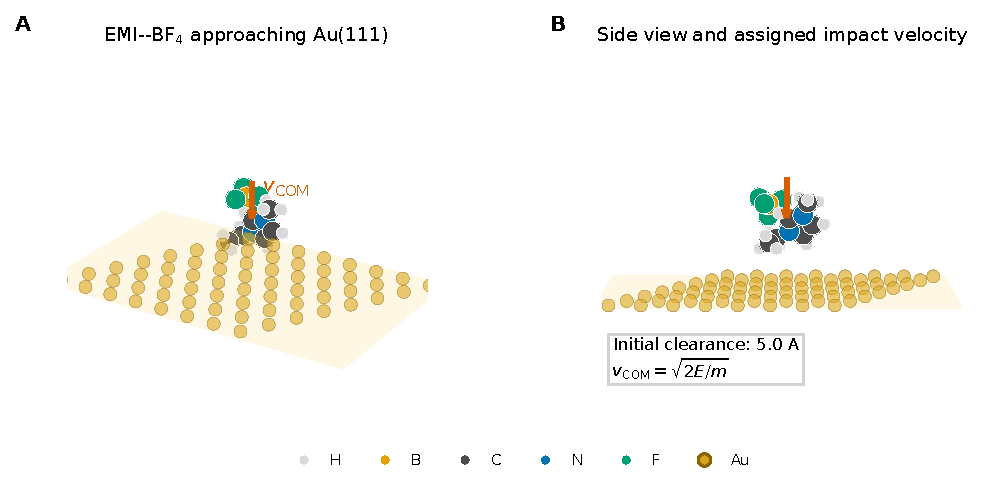
\includegraphics[width=\linewidth]{fig1_collision_setup.pdf}
  \caption{Initial wall-collision geometry. (a) Perspective view of the
  neutral EMI--BF$_4$ projectile above the frozen Au(111) slab used by the
  archived MACE-medium workflow. (b) Side view showing the 5-\AA{} initial
  clearance and surface-normal center-of-mass velocity. For projectile mass
  \(m\) and prescribed laboratory-frame impact energy \(E\), the assigned
  speed is \(v_{\mathrm{COM}}=\sqrt{2E/m}\); the seven energies span
  10--100~eV. The DFT/MM reference also uses an explicit frozen Au surface,
  whereas matched ReaxFF and MACE-POLAR-1 replace Au with continuum and
  harmonic repulsive wall potentials, respectively.}
  \label{fig:collision_setup}
\end{figure}

\subsection{Fragment identification and cross-method comparison}
\label{sec:fragment_analysis}

Molecular connectivity was reconstructed with element-pair cutoffs equal to
1.3 times the sum of ASE covalent radii. A neutral EMI--BF$_4$ ion pair
initially contains two covalently connected components; terminal states
containing more than two components were classified as covalently fragmented.
Connected components supplied molecular formulae and nominal masses. HF
formation was evaluated separately in every stored frame and at the terminal
frame. MACE trajectories were stored every 5~fs and ReaxFF trajectories every
50~fs. The ReaxFF analysis therefore excludes persistent or repeatedly sampled
HF but cannot exclude an intermediate shorter than the output interval.

Published DFT product masses and probability densities were digitized from
Fig.~7 of Laws and Petro \cite{Laws2026}, with estimated uncertainties of
\(\pm0.5\)~amu and \(\pm0.005\) probability-density units. Those bars pool
terminal fragments from six trajectories at each energy and do not yield exact
trajectory-level HF frequencies. We therefore compare DFT spectral evidence,
local trajectory incidence, and published ReaxFF product assignments as
distinct observables rather than treating them as equivalent reaction
probabilities.

\subsection{Computational benchmark}
\label{sec:benchmark_method}

ReaxFF wall time was measured for the complete 42-case matrix on one Intel
i9-13900K CPU thread per trajectory and includes process startup. MACE wall
times were projected from median local force-evaluation times multiplied by
4,000 force calls on an NVIDIA RTX~4090; model loading was excluded. The
DFT/MM value is the maximum reported by Laws and Petro, up to 60~days per
microcanonical trajectory on 16 CPU cores and 128~GB, rather than a mean
\cite{Laws2026}. Speedups are consequently order-of-magnitude throughput
comparisons, not hardware-normalized performance metrics.

\section{Results}
\label{sec:results}

\subsection{Energy-resolved product spectra}
\label{sec:spectra_results}

The mass spectra show the common progression from a small number of heavy
products at low energy to increasingly populated low-mass channels at high
energy (Fig.~\ref{fig:mass_spectra}). The comparison follows the
energy-stacked presentation used for the published DFT/MM and ReaxFF spectra
\cite{Bendimerad2022,Laws2026}. DFT/MM retains strong ion-pair products near
87 and 111~amu at 10~eV and develops a broader light-fragment distribution by
100~eV. The matched ReaxFF rerun is already rich in low-mass products at
10~eV, consistent with its earlier fragmentation onset. Both MACE spectra
shift toward lower mass with energy, but MACE-POLAR-1 retains a more discrete
set of intermediate-mass products than ReaxFF over much of the sampled range.

Peak heights in Fig.~\ref{fig:mass_spectra} are normalized independently
within each method--energy panel because the source quantities are not
identical: DFT/MM reports digitized probability density, whereas the local
models report fragment-occurrence frequency. The figure therefore supports
comparison of mass channels and spectral broadening, not absolute product
yields.

\begin{figure}[p]
  \centering
  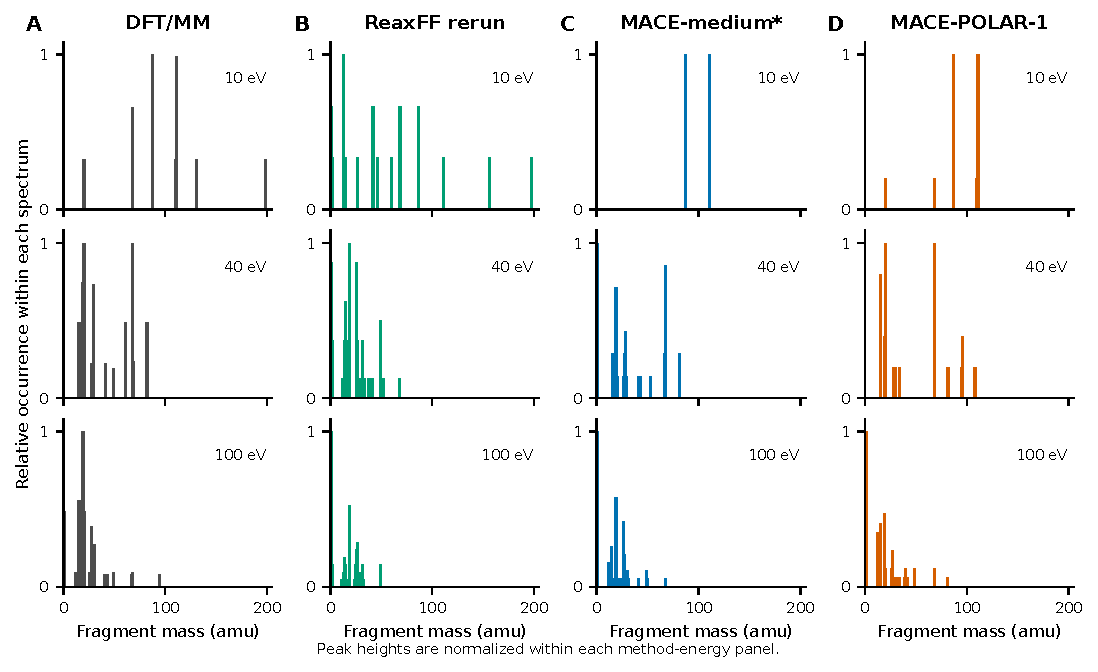
\includegraphics[width=\linewidth]{fig1_selected_mass_spectra.pdf}
  \caption{Fragment mass spectra at 10, 40, and 100~eV for published DFT/MM,
  the matched ReaxFF rerun, provisional MACE-medium, and MACE-POLAR-1.
  Each spectrum is normalized to its largest peak to emphasize product masses
  and broadening with impact energy. DFT/MM values were digitized from Laws
  and Petro Fig.~7 \cite{Laws2026}; local spectra were calculated from the six
  terminal trajectories at each energy.
  MACE-medium is marked with an asterisk because its archived Au--projectile
  wall interaction did not evaluate the intended pair parameters.}
  \label{fig:mass_spectra}
\end{figure}

\subsection{Fragmentation onset and orientation dependence}
\label{sec:fragmentation_results}

All three approximate methods generated progressively lighter products with
increasing collision energy and recovered common fluoroborate families
including BF$_4$, BF$_3$, BF$_2$, and F. The trajectory-level maps in
Fig.~\ref{fig:outcome_maps} retain the orientation dependence that is hidden
by energy-averaged curves.
The provisional MACE-medium ensemble retained the original covalent components
in all six 10-eV trajectories, but fragmented in five of six cases at 20~eV
and all cases from 30~eV upward. MACE-POLAR-1 fragmented in one of six cases
at 10~eV, five of six at 20~eV, and all cases from 30~eV. ReaxFF predicted the
earliest onset, with fragmentation in four of six 10-eV cases, five of six at
20~eV, and all cases from 30~eV.

These onset distributions do not reproduce the DFT/MM regime boundaries.
Laws and Petro \cite{Laws2026} associated 10--20~eV primarily with ionic
dissociation, 30--40~eV with neutralization, and prevalent covalent
fragmentation with energies above 50~eV. The discrepancy is important for
propulsion modeling because premature breakup changes the predicted number,
mass, and likely angular spread of secondary products. Agreement among
approximate methods at 20--30~eV is not independent validation; it instead
identifies compressed contacts, stretched ion pairs, and incipient bond
cleavage in the 10--40-eV interval as high-priority configurations for new DFT
labels.

\begin{figure}[htbp]
  \centering
  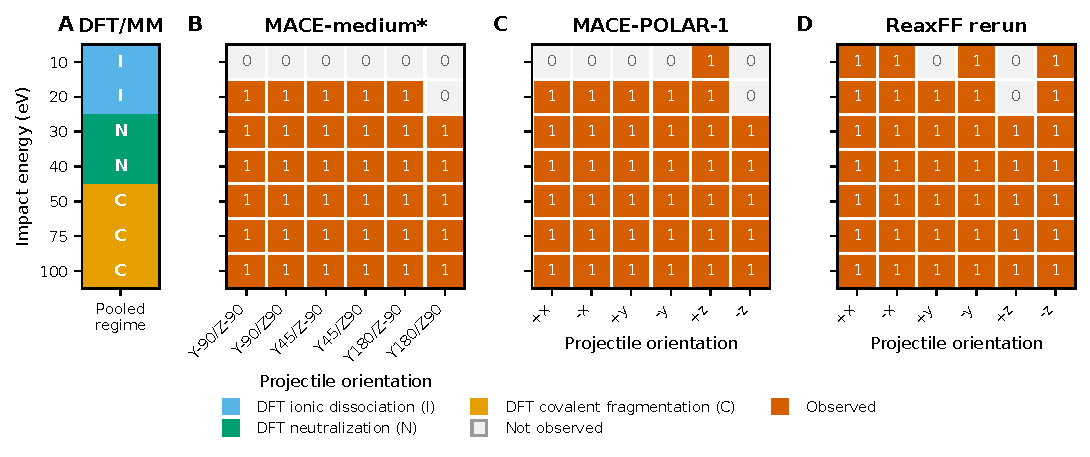
\includegraphics[width=\linewidth]{fig2_fragmentation_maps.pdf}
  \caption{Energy and orientation dependence of collision outcomes.
  (a) Dominant pooled DFT/MM regimes reported by Laws and Petro
  \cite{Laws2026}: ionic dissociation (I), neutralization (N), and covalent
  fragmentation (C). The DFT/MM paper does not publish trajectory-level
  outcomes by orientation. (b--d) Covalent-breakup outcomes for each local
  trajectory, where 1 and orange denote observed breakup. The format follows
  the landing-configuration maps of Bendimerad and Petro
  \cite{Bendimerad2022}. MACE-POLAR-1 and ReaxFF use the six Cartesian dipole
  orientations; archived MACE-medium uses its original Euler-rotation set.
  The asterisk denotes the provisional MACE-medium wall implementation.}
  \label{fig:outcome_maps}
\end{figure}

\subsection{Product-family comparison}
\label{sec:product_results}

\begin{figure}[htbp]
  \centering
  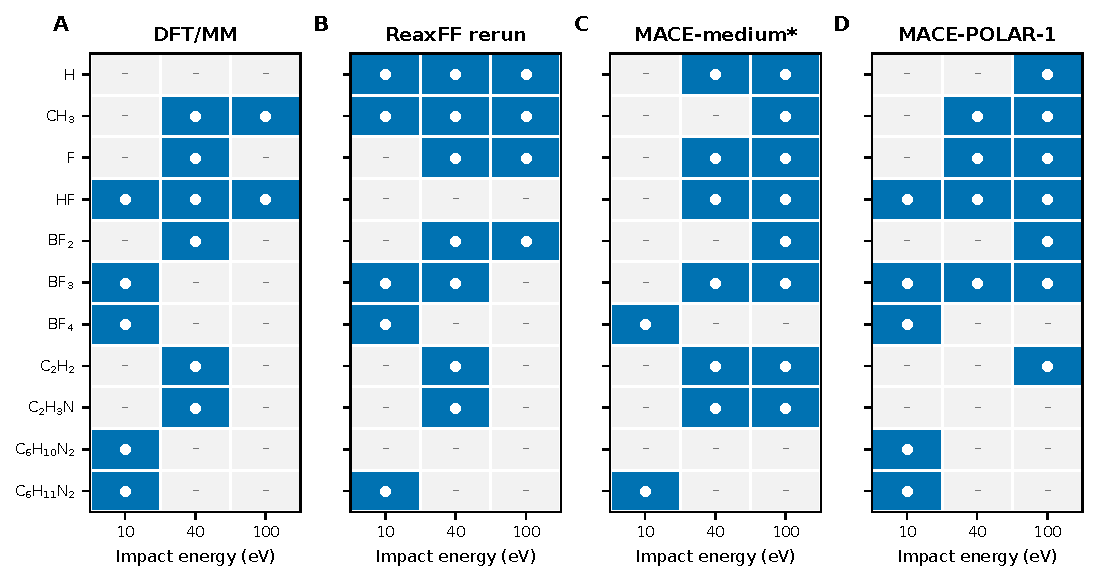
\includegraphics[width=\linewidth]{fig3_product_family_comparison.pdf}
  \caption{Occurrence of selected terminal product families at 10, 40, and
  100~eV. Filled cells indicate that the formula is reported in the published
  DFT/MM spectrum or occurs in at least one of the six local trajectories.
  The binary map compares chemical coverage rather than yield. Formulae are
  assigned from DFT/MM annotations or geometric connectivity in the local
  trajectories; electronic charge states are not available for the local
  models. The asterisk denotes provisional MACE-medium results.}
  \label{fig:product_families}
\end{figure}

Figure~\ref{fig:product_families} separates formula-level agreement from
nominal-mass overlap. All methods recover fluoroborate products, but their
energy dependence differs. DFT/MM retains BF$_4$ and BF$_3$ at 10~eV, adds
BF$_2$ and several light organic products at 40~eV, and is dominated by
lighter products at 100~eV. ReaxFF produces atomic H and CH$_3$ across the
selected energies and lacks a molecular HF assignment. MACE-medium and
MACE-POLAR-1 recover BF$_3$, F, and hydrocarbon fragments at elevated energy;
both also form HF. These are product-presence comparisons, not branching
ratios.

\subsection{Computational throughput}
\label{sec:throughput_results}

The matched ReaxFF trajectories required a measured mean of 1.37~s per 2-ps
trajectory on one CPU thread. Projected times were 2.54~min for MACE-medium
and 5.12~min for MACE-POLAR-1 on an RTX~4090. Laws and Petro
\cite{Laws2026} reported up to 1,440~h for one DFT/MM trajectory on 16 CPU
cores. Relative to that reported upper bound, the projected speedups are
approximately \(3.4\times10^4\) for MACE-medium and \(1.7\times10^4\) for
MACE-POLAR-1; ReaxFF is approximately \(3.8\times10^6\) times faster.

\begin{table}[htbp]
\centering
\caption{Computational wall time for a nominal 2-ps trajectory.}
\label{tab:performance}
\begin{tabularx}{\linewidth}{@{}lXr@{}}
\toprule
Method & Time per 2-ps trajectory & Speedup vs.\ DFT maximum \\
\midrule
DFT/MM       & Up to 1,440 h (16 CPU cores) & 1 \\
ReaxFF       & 1.37 s (one CPU thread)       & \(3.8\times10^6\) \\
MACE-medium  & 2.54 min (RTX 4090)           & \(3.4\times10^4\) \\
MACE-POLAR-1 & 5.12 min (RTX 4090)           & \(1.7\times10^4\) \\
\bottomrule
\end{tabularx}
\end{table}

A serial 42-case matrix would require up to 6.9~years if every DFT/MM
trajectory reached the reported maximum, compared with approximately 1.8~h
for MACE-medium, 3.6~h for MACE-POLAR-1, and 58~s for ReaxFF. These totals are
illustrative upper-bound or projected estimates rather than measured
end-to-end campaign times. Nevertheless, they establish the practical
hierarchy: ReaxFF supports very large statistical ensembles, DFT/MM supplies
the highest-fidelity reference chemistry, and MACE can make
energy--orientation ensembles tractable while retaining a reactive channel
absent from the tested force field.

\section{Discussion}
\label{sec:discussion}

\subsection{Implications for electrospray plume--surface modeling}
\label{sec:propulsion_implications}

The comparison places transferable MACE potentials in a useful intermediate
regime between ReaxFF sampling and DFT/MM chemistry. ReaxFF reproduces the
broad energy-to-mass trend at negligible trajectory cost, but the tested
description fragments too readily at low energy and produces a congested
low-mass spectrum before the DFT/MM covalent-fragmentation regime.
MACE-medium and MACE-POLAR-1 also shift fragmentation to lower energy than
DFT/MM, but retain a broader combination of fluoroborate, organic, and neutral
products. MACE-POLAR-1 is particularly relevant because its long-range terms
provide a physically motivated representation of ionic separation and
induction.

For electrospray diagnostics, this distinction is not cosmetic. Charged
secondary species can be sampled by TOF-SIMS or current-based diagnostics,
whereas BF$_3$, HF, and neutralized imidazolium products require a
neutral-sensitive measurement such as a residual gas analyzer
\cite{Laws2026,Shaik2024}. A model that reproduces only nominal fragment mass
can therefore miss the chemical partition between charged and neutral products
that drives suppression bias and background-gas composition. Likewise,
premature fragmentation would overpredict the number of light products, which
DFT/MM associates with broader deflection angles and diffuse contamination
\cite{Laws2026}. A validated machine-learned potential could supply the
trajectory statistics needed to pass energy- and orientation-dependent product
distributions into multiscale plume-interception and facility-effect models.

\subsection{Novelty and fine-tuning strategy}
\label{sec:fine_tuning}

The principal advance of this work is not a claim that an off-the-shelf
foundation model has replaced DFT/MM. It is the demonstration that a
transferable machine-learned potential can access a chemically specific,
propulsion-relevant neutralization product that the tested ReaxFF model
misses, while reducing the reported ab initio trajectory cost by roughly four
orders of magnitude. The same benchmark exposes a quantitative failure---the
early onset of covalent fragmentation---that defines a concrete route to
improvement. Capability, error, and computational value are thus evaluated in
the same collision matrix rather than inferred from equilibrium force errors
alone.

MACE-POLAR-1 is the preferred foundation for collision-specific refinement. A
targeted dataset should sample intact and ionically separating pairs at
10--20~eV; B--F cleavage, proton transfer, BF$_3$--HF formation, and competing
neutralization channels at 30--40~eV; and strongly compressed contacts with
diverse covalent products at 50--100~eV. Reference calculations should include
energies, forces, dipoles, and charge-sensitive observables where
methodologically consistent. Active learning can prioritize configurations on
which independently initialized models disagree, concentrating expensive
DFT/MM labeling near reaction boundaries rather than uniformly along
trajectories.

Validation should use complete held-out trajectories and unseen orientations.
The acceptance criteria should include the DFT/MM fragmentation regime
boundaries, ion-pair separation, HF formation and persistence, product-family
distributions, conservation behavior, and force stability during high-energy
contact. Surface fidelity must also be improved: a production model should
include verified Au--projectile interactions and, ultimately, mobile or
polarizable surface layers. ReaxFF, the corrected MACE-medium workflow, and
unfine-tuned MACE-POLAR-1 should remain fixed baselines so that improvements
can be attributed to the new labels rather than protocol changes.

\subsection{Limitations}
\label{sec:limitations}

The present comparison is heterogeneous by construction. MACE-medium,
MACE-POLAR-1, ReaxFF, and DFT/MM use different surface representations, and the
MACE-POLAR-1 trajectories are shorter and may end at a separation threshold.
The archived MACE-medium Au--projectile interaction was not evaluated as
intended and its values are provisional. The DFT/MM Au slab is also rigid,
suppressing surface-phonon energy accommodation and explicit
metal--projectile electron transfer \cite{Laws2026}. Local fragment identities
are geometric and do not provide electronic charge states. Six orientations
per energy do not define converged branching probabilities, ReaxFF output
spacing could miss very short-lived HF, and no new DFT/MM labels were
generated here. These limitations permit a comparison of observed chemical
channels, regime trends, and computational scale, but not quantitative ranking
of product yields or surface-specific accuracy.

The next stage should first correct the MACE-medium wall implementation and
then fine-tune MACE-POLAR-1 against collision-specific DFT/MM data. Extension
to collision-induced fragmentation by N$_2$ should follow only after the
surface-impact regime boundaries are validated. Gas-phase EMI$^+$, BF$_4^-$,
and solvated-cluster collisions would then test whether the learned
bond-breaking and proton-transfer chemistry transfers across the two
collisional environments relevant to electrospray plume evolution.

\section{Conclusions}
\label{sec:conclusions}

This benchmark evaluates transferable MACE foundation models against the
complementary strengths and limitations of published ReaxFF and DFT/MM
descriptions of neutral EMI--BF$_4$ surface impacts. ReaxFF provides the
highest throughput and reproduces the trend toward lighter products at higher
impact energy, but predicts extensive low-mass products at energies where
DFT/MM emphasizes ionic dissociation. Both MACE models reproduce the broad
spectral shift and multiple DFT-reported product families, including
fluoroborates, organic fragments, and HF. At the same time, all approximate
models fragment below the DFT/MM regime boundary, and the current surface
models are not equivalent. The results therefore support MACE-POLAR-1 as a
foundation for refinement, not as a quantitatively validated replacement for
DFT/MM.

At projected trajectory times of minutes rather than the reported DFT/MM
maximum of months, a fine-tuned polarizable MACE model could make
orientation-resolved reactive ensembles practical for SSE and facility-effect
studies. The immediate research target is a DFT/MM training and validation set
that constrains low-energy ionic dissociation, the 30--40-eV BF$_3$--HF
neutralization channel, and high-energy covalent fragmentation while
incorporating a verified extractor-surface interaction. Such a model would
connect ab initio reaction fidelity to the trajectory statistics required for
electrospray-thruster lifetime and diagnostic-correction models.

\section*{Data availability}

The release package contains digitized literature data, normalized local
summaries, analysis scripts, figure-generation code, and provenance records.
Raw trajectories are retained locally and excluded from the public Git
repository because of size. Archival publication should deposit the raw
trajectories and checksums in a versioned repository with a DOI.

\section*{Code availability}

The accompanying package includes scripts for the matched ReaxFF campaign,
trajectory normalization, fragment analysis, HF tracking, and figure
generation. Environment specifications, model identifiers, and software
licenses will accompany the public release.

\section*{CRediT authorship contribution statement}

\textbf{First Author:} Conceptualization, Methodology, Software, Validation,
Formal analysis, Investigation, Data curation, Visualization, Writing --
original draft. \textbf{Second Author:} [roles to be completed].
\textbf{Corresponding Author:} Supervision, Resources, Project administration,
Funding acquisition, Writing -- review and editing.

\section*{Declaration of competing interest}

The authors declare that they have no known competing financial interests or
personal relationships that could have appeared to influence the work
reported in this paper.

\section*{Acknowledgements}

[Add funding agencies, grant numbers, computing resources, and contributors.]

\bibliographystyle{elsarticle-num}
\bibliography{../references/references}

\end{document}
